\chapter{Relativity and Electromagnetism}
Classical electromagnetism is consistent with special relativity. Maxwell's equations are invariant under a Lorentz transformation and do not need to be modified. Indeed, Lorentz originally arrived at his transformation equations by requiring the invariance of Maxwell's equations. 

Relativity gives us a new point of view that enhances our understanding of electromagnetism. And the techniques of relativity are often much simpler than the classical techniques for solving electromagnetic problems, so that relativity theory is also a practical aid in problem solving.

\section{The Interdependence of Electric and Magnetic Fields}
Consider a charge that is in motion in an inertial reference frame $S$. This charge, which we may call the source charge $q_{8}$, sets up a field of magnetic induction $B$. Let another charge, called a test charge $q_{t}$, move through this field with a velocity $u$. Then the test charge will experience a magnetic force $\mathbf{F}_{m}=q_{t}(\mathbf{u} \times \mathbf{B})$ in the $S$-frame. Now, consider an observer in an inertial frame $S^{\prime}$ which moves relative to $S$, either with the velocity $u$ of the test charge or with the velocity of the source charge in $S$. In either one of these frames there will be no magnetic force, for either the velocity of the test charge is zero, or the source charge is at rest and there is no magnetic field; hence, $\mathbf{F}_{m}{ }^{\prime}=0$. But inertial frames are equivalent; none is preferred over another. Then is there or isn't there a magnetic force? The resolution of this paradox is simple in relativistic terms.

Paradoxes such as the one just raised are resolved by the fact, shown so clearly in relativity, that magnetic fields and electric fields have no separate meaning; instead, we have the single concept of an electromagnetic field. A field that is purely electric, or purely magnetic, in one frame, for example, will have both electric and magnetic components in another frame, in general. 
\section{Transformation of Charge and Current Densities}
We begin by considering a volume element containing charge. For simplicity, let the volume element be a cube whose edges have rest length $l_{0}$ and let there be $N$ electrons in the cube. The charge in the cube is $N e$, then, and the charge density (the charge per unit volume) is $\rho_{0}=$ $N e / l_{0}^{3}$. If the charges are at rest in frame $S^{\prime}$ then there will be no current in $S^{\prime}$ and the current density (current per unit cross-sectional area) will be $j_{0}=0$. Now, consider the volume element from a frame $S$ in which it moves with velocity $\mathbf{u}$. Again, for simplicity, take $\mathbf{u}$ to be in the direction of one edge of the cube. This edge will have the measured length $l_{0} \sqrt{1-u^{2} / c^{2}}$ in $S$ whereas the transverse edges will measure $l_{0}$ each. Hence, the volume of the cube in $S$ is $l_{0}^{3} \sqrt{1-u^{2} / c^{2}}$. However, the number of electrons and the charge on each do not change, so that the $S$ observer will find a charge density 
\begin{align*}
\rho&=N e / l_{0}^{3} \sqrt{1-u^{2} / c^{2}}.\text{ Combining this with $\rho_{0}$, we obtain}\\
\rho&=\frac{\rho_{0}}{\sqrt{1-u^{2} / c^{2}}} .\\
\intertext{The charges move with the velocity $u$ in $S$ so that $j$, the measured current density there (the current per unit cross-sectional area), will be the charge density of the cube times the velocity of the cube; that is, $j=\rho u=N e u / l_{0}^{3} \sqrt{1-u^{2} / c^{2}}$. Combining this with $\rho_{0}$, we obtain}
j&=\frac{\rho_{0} u}{\sqrt{1-u^{2} / c^{2}}} .
\intertext{If we had considered a current density $\mathbf{j}$ with components $j_{x}, j_{y}$, and $j_{z}$, we obviously would have obtained the general result}
j_{x} &=\frac{\rho_{0} u_{x}}{\sqrt{1-u^{2} / c^{2}}}, & j_{y}=\frac{\rho_{0} u_{y}}{\sqrt{1-u^{2} / c^{2}}} \\
j_{z} &=\frac{\rho_{0} u_{z}}{\sqrt{1-u^{2} / c^{2}}}, & \rho=\frac{\rho_{0}}{\sqrt{1-u^{2} / c^{2}}}
\end{align*}
Now we notice a very interesting analogy. The relation between current density and charge density is similar to that between momentum and energy and to that between space and time coordinates. In fact, just as $c^{2} t^{2}-\left(x^{2}+y^{2}+z^{2}\right)$ is an invariant quantity equal to $c^{2} \tau^{2}$, and just as $c^{2} m^{2}-\left({p_{x}}^{2}+p_{y}^{2}+p_{z}{ }^{2}\right)$ is an invariant quantity equal to $c^{2} m_{0}^{2}$ (see Problem 3-40, for example), so we can analogously derive an invariant quantity formed from $\mathbf{j}$ and $\rho$. It is easily shown (Problem 4-1) that $c^{2} \rho^{2}-\left(j_{x}^{2}+j_{y}^{2}+j_{z}^{2}\right)=c^{2} \rho_{0}^{2}$. The three analogous relations above may be written simply as
\begin{align*}
c^{2} t^{2}-r^{2} &=c^{2} \tau^{2} \\
c^{2} m^{2}-p^{2} &=c^{2} m_{0}^{2} \\
c^{2} \rho^{2}-j^{2} &=c^{2} \rho_{0}^{2}\\
\text{ and In fact, Eqs. 4-1 and }&\text{4-2 can also be written as}\\
\rho=\frac{\rho_{0}}{m_{0}} m \quad \text { and } \quad \mathbf{j}&=\frac{\rho_{0}}{m_{0}} \mathbf{p} .
\intertext{We see at once then that the quantities $\mathbf{j}$ and $\rho$ transform exactly as $p$ and $m$, respectively. Hence we obtain the transformation equations}
j_{x}^{\prime}&=\frac{j_{x}-\rho v}{\sqrt{1-v^{2} / c^{2}}}, \quad j_{y}^{\prime}=j_{y}, \quad j_{z}{ }^{\prime}=j_{z} \\
\rho^{\prime}&=\frac{\rho-j_{x} / c^{2}}{\sqrt{1-v^{2} / c^{2}}}\\
\text{and their }&\text{inverses}\\
j_{x}&=\frac{j_{x}{ }^{\prime}+\rho^{\prime} v}{\sqrt{1-v^{2} / c^{2}}}, \quad j_{y}=j_{y}^{\prime}, \quad j_{z}=j_{z}^{\prime}, \\
\rho&=\frac{\rho^{\prime}+v j_{x}{ }^{\prime} / c^{2}}{\sqrt{1-v^{2} / c^{2}}}
\end{align*}
As usual, we assume that frame $S^{\prime}$ moves with a velocity $v$ with respect to frame $S$ along their common $x-x^{\prime}$ axes.)
\begin{exercise}
 Consider a long straight wire (frame S) in which free electrons move with a (drift) velocity $u$ to the right. We take the number of free electrons per unit volume, $n$, to be equal to the number of positive ions per unit volume, so that the net charge in any volume element of the wire is zero. The positive charge, however, is at rest in frame $S$ whereas the electrons are in motion\\
 \textbf{(a) }Write down the chatge density and the current density in $S$\\
 \textbf{(b) }Consider the situation in $S^\prime$, an inertial frame moving with speed $v$ to the right relative to $S$. Write down the chatge density and the current density in $S^\prime$
 \begin{figure}[H]
 	\centering
 	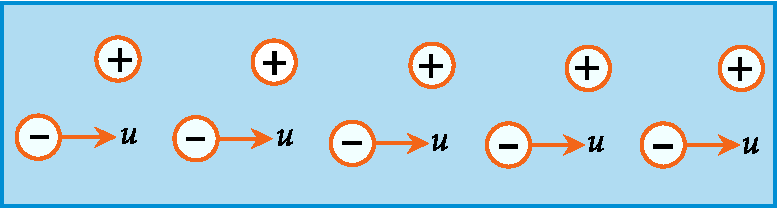
\includegraphics[height=2cm,width=7cm]{R-1}
 	\caption{}
 	\label{}
 \end{figure}
\end{exercise}
\begin{answer}
	\textbf{(a) }
	\begin{align*}
	\text{The negative-charge density(caused by electrons )is }\rho^-&=-ne, \\
	\text{ Where $e$ is the magnitude of an }&\text{electronic charge,}\\
	\text{Whereas the positive-charge density(caused by the ions) is }\rho^+&=+ne\\
	\text{The net charge density, }\rho&=\rho^-+\rho^+=0\\
	\text{As for the current density we have }{j_z}^-&=-neu=\rho^-u\\
	\text{and }{j_z}^+=0, \text{ so that }j_z&={j_z}^++{j_z}^-=\rho^-u
	\end{align*}
	\textbf{(b) }
	\begin{align*}
	\intertext{ For an observer in $S^\prime$ the positive charge is in motion to the left also he will find the wire is not electriclly neutral}
	\text{The charge   }&\text{density in $S^\prime$}\\
	\rho^{-\prime}&=\frac{\rho^{-}-v j_{x}^{-} / c^{2}}{\sqrt{1-v^{2} / c^{2}}} \quad \text { and } \quad \rho^{+\prime}=\frac{\rho^{+}-v j_{x}^{+} / c^{2}}{\sqrt{1-v^{2} / c^{2}}}\\
	\text { and with } j_{x}^{-}&=\rho^{-} u \text { and } j_{x}^{+}=0 \text {, we obtain }\\
	\rho^{-\prime}&=\rho^{-} \frac{\left(1-v u / c^{2}\right)}{\sqrt{1-v^{2} / c^{2}}} \quad \text { and } \quad \rho^{+^{\prime}}=\frac{\rho^{+}}{\sqrt{1-v^{2} / c^{2}}}\\
\text{	Substituting }\rho^{-}&=-n e\text{ and }\rho^{+}=+n e,\text{ we get for the net charge density,} \left[\rho^{\prime}=\rho^{+^{\prime}}+\rho^{-\prime}\right]\\
\rho^{\prime}&=\frac{n e}{\sqrt{1-v^{2} / c^{2}}}-\frac{n e\left(1-v u / c^{2}\right)}{\sqrt{1-v^{2} / c^{2}}}=-\frac{n e v u / c^{2}}{\sqrt{1-v^{2} / c^{2}}}\\
\text{which is positive }&\text{and not zero. The primed observer finds the wire to be positively charged.}\\
\text{Similarly the current}&\text{ density}\\
{j_x}^{-\prime}&=\frac{{j_x}^--v\rho^-}{\sqrt{1-v^{2} / c^{2}}}=\frac{-neu-v(-ne)}{\sqrt{1-v^{2} / c^{2}}}\\
{j_x}^{-\prime}&=\frac{-ne(u-v)}{\sqrt{1-v^{2} / c^{2}}}\\
{j_x}^{+\prime}&=\frac{{j_x}^+-v\rho^+}{\sqrt{1-v^{2} / c^{2}}}=\frac{-vne}{\sqrt{1-v^{2} / c^{2}}}\\
{j_x}^{\prime}&=\frac{-neu}{\sqrt{1-v^{2} / c^{2}}}
\end{align*}
\end{answer}
\section{The Transformation for $E$ and $B$}
The electromagnetic (or Lorents ) force on a particle of charge $q$ moving with velocity $u$, at a point and a time ar which the electric field is $E$ and the magnetic field is $B$,is  
$$F=q(E+u\times B)$$
Although the electric force does not depends on the motion of the test charge, the magnetic force does. However, the motion of a particle depends on the frame in which it is described, so that we should not be surprised that the fields also depends on the frame in which they are described. We shall derive the field transformations here from special cases, the resuts, however, being quite generally true. \\
Force transformation equations between a frame $S$ and another frame $S^\prime$, in which the particle experiencing the force is instantaneously at rest, is
	\begin{align*}
	F_x&={F_x}^{\prime}\\
	F_y&={F_y}^{\prime}\sqrt{1-v^{2} / c^{2}}\\
	F_z&={F_z}^{\prime}\sqrt{1-v^{2} / c^{2}}
	\end{align*}
Consider a particle of charge q to be instantaneously at rest in $S^\prime$, where in there is an electric field $E^\prime$ and a magnetic field $B^\prime$. The electromagnetic force on the particle will be $F^\prime=qE^\prime$, there being no magnetic force on a particle at rest. In frame $S$ the corresponding force is given by $F=q(E+v\times B),$ for in this frme the charge has a velocity $v$, the velocity of $s^\prime$ relative to $S$. We take $v$ to be along the common $x-x^\prime$ axes so that $v_z=v$ and $v_y=v_z=0.$\\
 We find, with $(v \times B)_{x}=$ $v_{y} B_{z}-v_{z} B_{y}=0$, that $F_{x}=q\left[E_{x}+(\mathbf{v} \times \mathbf{B})_{x}\right]=q E_{x}$ and $F_{x}^{\prime}=q E_{x}^{\prime}$. Then, the equation $F_{x}^{\prime}=F_{x}$ gives us $q E_{x}^{\prime}=q E_{x}$, and we have
 \begin{align*}
 E_{x}{ }^{\prime}&=E_{x}
 \intertext{as the transformation equation for $E_{x}{ }^{\prime}$.
 Using the $y$-component equation, we obtain $q E_{y}{ }^{\prime} / \gamma=q\left[E_{y}+(\mathbf{v} \times \mathbf{B})_{v}\right]$ or, since $(\mathbf{v} \times \mathbf{B})_{v}=v_{z} B_{x}-v_{x} B_{z}=-v B_{z}$, the transformation equation for $E_{v}{ }^{\prime}$ is}
 \boldsymbol{E}_{\nu}{ }^{\prime}&=\gamma\left(\boldsymbol{E}_{\nu}-v \boldsymbol{B}_{z}\right) .\\
 \text{Similarly, from the $z$-component}&\text{ equation we obtain the transformation equation for $E_{z}{ }^{\prime}$, namely}\\
 E_{z}{ }^{\prime}&=\gamma\left(E_{z}+v B_{y}\right) .\\
\text{ Hence, we can summarize the }&\text{transformation for the electric field components as}
 \end{align*}
\renewcommand*{\arraystretch}{1.5}
$$\begin{array}{ll}E_{x}^{\prime}=E_{x} & E_{x}=E_{x}{ }^{\prime} \\ E_{y}^{\prime}=\gamma\left(E_{y}-v B_{z}\right) & E_{y}=\gamma\left(E_{y}{ }^{\prime}+v B_{z}{ }^{\prime}\right) \\ E_{z}^{\prime}=\gamma\left(E_{z}+v B_{y}\right) & E_{z}=\gamma\left(E_{z}{ }^{\prime}-v B_{y}{ }^{\prime}\right)\end{array}$$\\
The force $\mathbf{F}=q(\mathbf{E}+u \times \mathbf{B})$ in $S$ has components $F_{x}=q\left(E_{x}+u_{y} B_{z}\right), \quad F_{y}=q\left(E_{y}-v B_{z}\right)$, and $F_{z}=q\left(E_{z}+\right.$ $\left.v B_{y}-u_{y} B_{x}\right)$\\
Now that we have the components of force in each inertial frame, we must substitute them into the general force transformation equations\\
 Hence, we can summarize the transformations for the magnetic field components as
$$
\renewcommand*{\arraystretch}{1.5}
\begin{array}{ll}
B_{x}{ }^{\prime}=B_{x} & B_{x}=B_{x}{ }^{\prime} \\
B_{y}{ }^{\prime}=\gamma\left(B_{y}+\frac{v}{c^{2}} E_{z}\right) & B_{y}=\gamma\left(B_{y}{ }^{\prime}-\frac{v}{c^{2}} E_{z}{ }^{\prime}\right) \\
B_{z}{ }^{\prime}=\gamma\left(B_{z}-\frac{v}{c^{2}} E_{y}\right) & B_{z}=\gamma\left(B_{z}{ }^{\prime}+\frac{v}{c^{2}} E_{y^{\prime}}\right) 
\end{array}
$$